
%CONFIGURACION DEL DOCUMENTO
\documentclass[12pt,spanish]{report}
\usepackage[spanish,activeacute]{babel}
\usepackage{epsfig}
\usepackage{setspace}
\usepackage{capt-of}
\oddsidemargin 0.2in
\textwidth 6.5in
\topmargin -0.25in
\textheight 9in
\pagestyle{myheadings}

\makeatletter
\long\def\@makecaption#1#2{
\vskip\abovecaptionskip
\sbox\@tempboxa{#1. #2}
\ifdim \wd\@tempboxa >\hsize
#1. #2\par
\else
\global \@minipagefalse
\hb@xt@\hsize{\hfil\box\@tempboxa\hfil}
\fi
\vskip\belowcaptionskip}
\makeatother


% INICIO DEL DOCUMENTO
\begin{document}
\doublespacing
\pagenumbering{roman}
\tableofcontents
%\listoffigures
%\listoftables
\newpage


\pagenumbering{arabic}
\chapter{Introducci\'on}
\newpage

\emph{LimeSurvey} permite a los usuarios crear de forma r'apida, potente e intuitiva, encuestas en las que pueden participar decenas de miles de participantes sin mucho esfuerzo, funcionando como auto-gu'ia para los encuestados que participan en las encuestas. Este manual se centra en c'omo crear, administrar y apoyar a los administradores y usuarios de la aplicaci'on.

El equipo de desarrollo de \emph{LimeSurvey} ha realizado grandes cambios y añadido nuevas caracter'isticas durante el desarrollo de la aplicaci'on en los 'ultimos años. Aseg'urese de actualizar a la ultima versi'on para poder hacer uso de todas las caracter'isticas que se resaltan en esta documentaci'on.
\newpage

\chapter{La encuesta}
\newpage

\section{Elementos b'asicos de una encuesta}

Una {\bf encuesta} tiene 3 elementos esenciales que deben aparecer siempre:

\begin{itemize}
\item Un nombre.
\item Al menos un grupo.
\item Al menos una pregunta.
\end{itemize}

Otros elementos opcionales en una nueva {\bf encuesta}  pueden ser:
\begin{itemize}
\item Respuestas aplicables para cada pregunta.
\item Subpreguntas, aplicables a preguntas.
\item Condiciones que determinan si una pregunta debe ser realizada.
\item Cuotas.
\item Entre otras muchas m'as.
\end{itemize}


\subsection{T'itulo de la encuesta}
\label{'titulo_encuesta'}
Proporciona un nombre 'unico para una encuesta, el cual se utiliza adem'as como opci'on en el listado de Encuestas para acceder a varias configuraciones aplicables a la encuesta como un todo. Opciones tales como el mensaje personalizado en la pantalla de bienvenida, la descripci'on de la encuesta, la informaci'on de contacto con el administrador de la encuesta, y la forma en que ser'an hechas las preguntas.


\subsection{Grupos de Preguntas}
\label{'grupo_preguntas'}
Una encuesta necesita que cada pregunta sea miembro de un grupo (y s'olo de ese grupo). Dependiendo del n'umero de preguntas en la encuesta, los {\bf Grupos} se pueden usar para definir secciones l'ogicas, tem'aticas en com'un, o posiblemente p'aginas por pantalla. Un grupo puede tener preguntas sobre un tema en particular o simplemente sea una agrupaci'on de preguntas que las haga m'as manejables.
Un grupo de preguntas tiene un t'itulo y una descripci'on opcional. Debe haber al menos uno en cada encuesta, incluso si no se desea dividir la encuesta en varios grupos.


\subsection{Preguntas}
\label{'preguntas'}
Las preguntas son el n'ucleo de la encuesta. No hay un l'imite real al n'umero de preguntas que puede haber en la encuesta o en un grupo. Las preguntas incluyen el texto mismo de la pregunta, as'i como la configuraci'on que determina qu'e tipo de respuesta aceptar'an. Es posible, adem'as, especificar un pequeño texto explicativo (ayuda) para cada pregunta y determinar si la pregunta es obligatoria u opcional. Para m'as detalles, revisar la secci'on tipos de preguntas ver en p'agina ~\pageref{'tipos_preguntas'}.

\newpage

\chapter{Interfaz administrativa}
\newpage
LimeSurvey presenta barras de herramientas horizontales al administrador de la encuesta en su navegador web. Estas barras representan cabeceras de varias ventanas (y sub ventanas) que permiten interacci'an con el sistema.


\section{Barra administrativa}
La primera barra que aparece es usualmente la {\bf Barra administrativa}, la cual permite ejecutar acciones de gesti'on a nivel global. De importancia son la lista desplegable de Encuestas junto con el bot'on de Crear Nueva (Encuesta), ambos en la parte derecha de la barra, estar'an disponibles si dicho usuario cuenta con los permisos adecuados.\\
\par
\centerline{\hbox{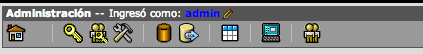
\psfig{file=barra_administrativa.png}}}
\captionof{figure}{Barra administrativa}
\par


Si la {\bf Barra administrativa} no aparece colocada en la parte superior, haga click en el bot'on Home  \hbox{
\psfig{file=icons/home.png}} para hacer que vuelva. 


Haciendo click en el bot'on Crear Nueva \hbox{
\psfig{file=icons/add.png}}  o seleccionando una encuesta ya existente, esto permite gestionar la Encuesta.

\newpage

\section{Barra de encuesta}
En el Grupo de preguntas, se puede hacer click en la lista desplegable de preguntas o en el bot'on Crear Nueva \hbox{
\psfig{file=icons/add.png}}   para agregar una cuarta barra de herramientas para editar la configuraci'on espec'ifica de una Pregunta.\\
\par
\centerline{\hbox{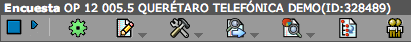
\psfig{file=barra_encuesta.png}}}
\captionof{figure}{Barra de encuesta}
\par

\section{Botones comunes}

En estas barras de herramientas anidadas existen algunos botones de navegaci'on en com'un. Hay un bot'on de Edici'on \hbox{
\psfig{file=icons/edit.png}}, 'util para editar el objeto que se ha seleccionado. Por defecto, aparecer'a en el navegador web el editor correspondiente al crear cualquier objeto. Tambi'en existe un bot'on de Borrado   \hbox{
\psfig{file=icons/delete.png}} para eliminar objetos en general. 
Para las barras de Grupos de Preguntas y Preguntas, hay un bot'on de Reordenado   \hbox{
\psfig{file=icons/organize_3.png}}  que cambia el orden en el cual dichos objetos aparecer'an al encuestado. 
Finalmente, est'a disponible un bot'on para Exportar  una encuesta   \hbox{
\psfig{file=icons/dumpquestion_2.png}},  grupo de preguntas o pregunta individual, que se puede importar de vuelta en otra encuesta diferente. Cabe hacer notar que el bot'on Crear  tambi'en permite importar un objeto previamente exportado.


Finalmente, hay dos a tres peque'nos botones en la esquina derecha de cada barra  para minimizar, maximizar y cerrar la ventana de la misma barra. El bot'on de maximizar llevar'a al usuario de vuelta a la vista de Resumen del objeto seleccionado actualmente.

Como es de suponer, la ventana a continuaci'on de la barra de herramientas activa ser'a minimizada de manera autom'atica al editar otro objeto de menor nivel dentro del actual. Solamente la barra de herramientas actualmente activa y su ventana pueden ser cerradas. Es posible abrir una barra de herramientas anterior que est'e minimizada presionando su bot'on de maximizar. Y se puede tambi'en ir directamente a de una a otra ventana seleccionando o creando un objeto nuevo en otra barra de herramientas sin tener que cerrar la actualmente abierta primero.



\chapter{Creando una encuesta}
\newpage

\section {Opciones de la encuesta}
Para crear una nueva encuesta presione el bot'on ``A'nadir' ' que se encuentra al lado derecho de la barra de ``Botones de Administraci'on' '. Aparecer'a una nueva ventana llamada ``Crear Nueva Encuesta' '. La mayor'ia de las preferencias se pueden editar m'as adelante presionando ``Editar Opciones de la Encuesta' ' en el men'u de ``Propiedades de la Encuesta' ' de la ``Barra de la Encuesta' '.\\

\subsection {Crear, importar o copiar encuesta}

Todas las preferencias y funciones est'an organizadas en pesta'nas. \\
A continuaci'on una descripci'on de cada pesta'na y campo.

\subsection {General}

\begin{enumerate}
	\item {\bf Idioma por omisi'on:}\\ 
	Establece el idioma base de la encuesta. Una vez grabado no se puede cambiar. Este idioma es la base para posibles traducciones de la encuesta. Durante la creaci'on de la encuesta no se pueden a'nadir idiomas, pero esto se puede hacer editando las propiedades de la encuesta una vez finalizada.
	
	\item	{\bf T'itulo:}\\ 
	Es un nombre breve y descriptivo para la encuesta. Este t'itulo estar'a presente en todas las páginas de la encuesta.
	
	\item {\bf Descripci'on: }\\
	Permite a'nadir una descripci'on de la encuesta. Se pueden incorporar elementos HTML como im'agenes o videos en esta secci'on utilizando el editor WYSIWYG. La descripci'on es incluida en el correo electr'onico de invitaci'on.
	
	\item {\bf Mensaje de Bienvenida:}\\
	Permite crear un mensaje que ser'a visible cuando el participante entre por primera vez a su encuesta. Se pueden incorporar elementos HTML como imágenes o videos en esta secci'on utilizando el editor WYSIWYG.
	
	\item {\bf Mensaje Final: }\\
	Permite crear un mensaje que ser'a visible cuando el participante finalice su encuesta. Se pueden incorporar elementos HTML como im'agenes o videos en esta secci'on utilizando el editor WYSIWYG.
	
	\item {\bf URL de salida:} \\ 
	Este URL estar'a presente como un enlace al final de la encuesta, lo cual permite redirigir al participante a cualquier p'agina en la web. Debe iniciar con ``http://' ' al principio. Puede usar \{SAVEDID\}, \{TOKEN\}, \{SID\} y \{LANG\} en el URL.\\
	\begin{itemize}
		\item SAVEDID es la identificaci'on de una encuesta en particular, TOKEN es utilizado para identificar a un participante en particular, SID es la identificaci'on de la encuesta como tal y LANG es el lenguaje del c'odigo.
		\item Ejemplo: \\
		.../info.php?var1=\{SAVEDID\}\&var2=\{TOKEN\}\&var3=\{SID\}\&lang=\{LANG\}
		\item De la versi'on 1.82 en adelante se pueden usar campos URL como por ejemplo\\ \{INSERTANS:SGQA\} en este URL Final. Esto permite a'nadir la respuesta a una pregunta espec'ifica al URL Final.
		\item Esto puede ser 'util para enviar una respuesta particular a un ``External Script' '. Tambi'en puede usar el nombre de un campo y relacionarlo a un valor en el URL. 
		\item En algunos casos usted podr'ia querer pasar un valor en el principio de la encuesta y despu'es utilizarlo en una ``External Script' ' al final. 
		\item En este caso usted empezar'ia la encuesta con el URL\\ ``index.php?sid=12345\&passthru=subsid\&subsid=9999' '.
		\item Luego utilizar'ia \{PASSTHRULABEL\} y \{PASSTHRUVALUE\} para reusar esos valores al final de la encuesta. 
		\item Un URL como 	``.../test.php?\{PASSTHRULABEL\}=\{PASSTHRUVALUE\}' ' se convertir'ia en ``.../test.php?subsid=9999' '.
	\end{itemize}
	\item {\bf Descripci'on del URL: } \\
	 Una descripci'on para el enlace del URL final.
	\item {\bf Formato de fecha: }\\
		Este es el formato que daremos a la salida de los reportes.
	\item {\bf Marca decimal: }\\
		Selecionamos nuestro tipo de decimal requerido.
	\item {\bf Administrador: } \\
		 Este es el nombre de la persona contacto quien administra la encuesta, ser'a incluido en correos electr'onicos enviados para invitar a los participantes.
	\item {\bf Correo Electr'onico del Administrador: } \\
		 Este es la direcci'on de correo electr'onico del administrador previamente definido. Cualquier respuesta a correos electr'onicos enviados llegara a esta direcci'on. Pueden ser varias direcciones separadas por punto y coma (;).
	\item {\bf Correo Electr'onico de Rebote: } \\
		 Esta es la direcci'on a la cual de haber un error de envío un mensaje es mandado. Usualmente es la misma direcci'on que la del administrador.
	\item {\bf Fax: } \\
	 	Este campo se utiliza para dar un n'umero de fax en la versi'on impresa de la encuesta.
	\paragraph{ Precauci'on: }
	 El editor HTML WYSIWYG no permite subir archivos durante la creaci'on de la encuesta. Si usted necesita subir l'aminas u otros recursos lo deben hacer despu'es de la creaci'on de la encuesta editando la misma.
\end{enumerate}


\section {Presentaci'on y Navegaci'on}



\begin{enumerate}
	\item {\bf Formato: } \\ Seleccione entre ``Preguntas por Preguntas' ', ``Grupo por Grupo' ' o ``Todas en una' '
	\begin{itemize}
		\item {\bf Preguntas por preguntas: } \\ Presentara una pregunta por p'agina.
		\item {\bf Grupo por grupo: } \\ Presentara un grupo de preguntas por p'agina. Tienen una p'agina de ``Bienvenida' ' y ``Env'io' ' separadas.
		\item {\bf Todas en una: } \\ Presentara todas las preguntas en la misma p'agina. NO tienen una p'agina de ``Bienvenida' ' y ``Env'io' ' separadas.
	\end{itemize}
	\item {\bf Plantilla: } \\ Seleccione una de las plantillas (templates) instaladas en su sistema.
	\item {\bf Mostrar pantalla de bienvenida: } \\ Seleccione Si o No para presentar el mensaje definido de Bienvenida.
	\item {\bf Retardo de navegaci'on: } \\ Selecciones la cantidad de segundos que el participante debe esperar para que los botones ``Anterior' ' y ``Pr'oximo' ' sean activados.
	\item {\bf Mostrar el bot'on ``Anterior' ': } \\ Seleccione Si o No para darle la opci'on al participante a moverse a p'aginas anteriores mientras completa la encuesta.
	\item {\bf Mostrar index de pregunta/permitir saltos: } \\ Seleccione Si o No para presentar a la derecha los n'umeros de las preguntas y permitir cambiar de una a otra.
	\item {\bf Operaci'on sin teclado: } \\ Seleccione Si o No para activar un teclado virtual cuando sea necesario.
	\item {\bf Mostrar la barra de progreso: } \\ Seleccione Si o No para ense'nar la barra de progreso
	\item {\bf Participantes pueden imprimir las respuestas: } \\ Seleccione Si o No para permitir que el usuario imprima un resumen de sus respuestas al finalizar la misma.
	\item {\bf Estad'isticas p'ublicas: } \\ Seleccione Si o No para que al finalizar la encuesta halla un enlace a las estad'isticas de la encuesta. Se pueden escoger que preguntas incluir.
	\item {\bf Presentar graficas en estad'isticas p'ublicas: } \\ Seleccione Si o NO para determinar si las estad'isticas presentan gr'aficas.
	\item {\bf Autom'aticamente acceder URL cuando la encuesta finalice: } \\ Seleccione Si o No para autom'aticamente llevar al usuario al URl Final establecido.
	\item {\bf Mostrar ``Hay X preguntas en la encuesta' ': } \\ Seleccione Si o No para ense'nar este mensaje en la Bienvenida.
	\item {\bf Mostrar los nombres/descripci'on de los grupos: } \\ Seleccione entre Ense'nar ambos, Ense'nar nombres solamente, Ense'nar descripci'on solamente, o Esconder ambos.
	\item {\bf Mostrar los n'umeros/c'odigos de las preguntas: } \\ Seleccione entre Ense'nar Ambos, Ense'nar n'umeros solamente, Ense'nar c'odigos solamente, o Esconder ambos.
	\item {\bf Mostrar ``No respuesta' ': } \\ Seleccione Si o No para permitir que el usuario no conteste preguntas opcionales.
\end{enumerate}

\subsection {Publicaci'on y Control de acceso}

	\begin {enumerate}
		\item {\bf Enlistar la encuesta p'ublicamente:}\\
			 Seleccione Si o No para enlistar la encuesta como ``Disponible' '.
		\item {\bf Fecha inicial:}\\
			 Seleccione la fecha y hora, si desea, en la que empezara la encuesta.
		\item {\bf Fecha de expiraci'on:}\\
			 Seleccione la fecha y hora, si desea, en la que expirar'a la encuesta.
		\item {\bf Utilizar cookies para prevenir la participaci'on repetida:}\\
			 Selecciones Si para prevenir que desde una misma computadora se hagan m'ultiples encuestas.
		\item {\bf Usar CAPTCHA para:}\\
			 Con esta opci'on usted selecciona cuando quiere usar un CAPTCHA.
	\end{enumerate}

\subsection {Notificaciones y Manejo de datos}

	\begin{enumerate}
		\item {\bf Mandar correo electr'onico de notificaci'on b'asica de administrador a:} \\
		Estos campos permiten enviar notificaciones a direcciones adicionales una vez la encuesta est'a finalizada. Las plantillas (templates) de estos correos electr'onicos se pueden editar. M'ultiples direcciones se separan con punto y coma (;). Hay tres formas de entrar direcciones:
		\begin{enumerate}
			\item Una direcci'on de correo electr'onico
			\item Un c'odigo SGQA para enviar el correo electr'onico a una direcci'on entrada como respuesta a una pregunta.
			\item Un c'odigo TOKEN (solo si la encuesta no es an'onima) para enviar a una direcci'on encontrada en un campo TOKEN con el formato \{TOKEN:EMAIL\} o \{TOKEN:ATTRIBUTE\_\_1\}.
		\end{enumerate}
		\item {\bf Marcar la fecha: }\\
			Seleccione Si o No para que todas las respuestas indiquen la fecha y hora en la que fueron contestadas.
		\item {\bf Guardar  la direcci'on IP: }\\
			Seleccione Si o No para que todas las respuestas indiquen el ``IPaddress' ' del participante.
		\item {\bf Guardar URL de referencia: }\\
			Seleccione Si o No para que todas las respuestas indiquen el URL del cual el participante acceso la encuesta.
		\item {\bf Guardar Tiempos: }\\
			Activar para crear una tabla con la cantidad de tiempo que el participante se tom'o para contestar cada pregunta.
		\item {\bf Activar modo de evaluaci'on: }\\
			Seleccione si activar o desactivar las evaluaciones para la encuesta.
		\item {\bf Participante puede guardar y continuar despu'es: }\\
			Seleccione Si o No para que el usuario pueda guardar sus respuestas y continuar despu'es, es m'as recomendable que se utilice en encuestas an'onimas.
		\item {\bf Google Analytics API  y Google Analytics styel: }\\
			Informacion sobre el uso de Google Analytics en nuestras encuestas.
	\end{enumerate}

\subsection{Participantes}
	\begin{enumerate}
		\item {\bf Respuestas an'onimas: }\\
			Esto permite escoger entre recopilar informaci'on de los participantes  o mantener la encuesta an'onima.
		\item {\bf Permitir editar respuestas despu'es de completar: }\\
			Esto permite que el usuario pueda re-acceder la encuesta mediante la invitaci'on y cambiar sus respuestas (solo funciona con encuestas no an'onimas).
		\item  {\bf Activar persistencia de respuestas basadas en participantes:} \\
			Esto permite que cada vez que el participante conteste una pregunta se grabe la encuesta autom'aticamente (solo funciona si la encuesta tiene participantes y no es an'onima).
		\item  {\bf Permitir registraci'on p'ublica: }\\
			Si usted utiliza particiantes en su encuesta las 'unicas personas que pueden acceder la misma son las que tienen usuario 'unico de la tabla de participantes. Si usted quiere utilizar TOKENS y permitir registraci'on publica seleccione esta opci'on. Esto permite que un visitante se registre con su nombre y correo electr'onico; se crear'a un participante nuevo para esta persona y luego se le enviar'a la invitaci'on.
		\item {\bf Usar formato HTML al enviar pases por correo electr'onico:}\\
			 Seleccione Si o No para que todos los correos electr'onicos enviados por la administraci'on de personas (invitaci'on, recordatorio, confirmaci'on) sean formateados con HTML.
		\item {\bf Ajustar tama'no de la contrase'na a : }\\
			El n'umero definido debe ser mayor que 5 y menor que 9.
	\end{enumerate}
	
\subsection{Importar}

Alternativamente usted puede importar una estructura de encuesta desde esta pestaña en ``Creaci'on de encuestas' '. Usted tiene la opci'on de permitir que LimeSurvey autom'aticamente convierta URLs relativos a im'agenes/media local y INSERTANS (recomendado).

\subsection {Copiar}

Alternativamente usted puede copiar una encuesta existente desde esta pesta'na en ``Creaci'on de encuestas' '. Usted tiene la opci'on de permitir que LimeSurvey autom'aticamente convierta URLs relativos a im'agenes/media local y INSERTANS (recomendado).


\subsection{Idiomas Adicionales}

Para a'nadir idiomas adicionales a una encuesta, esta debe ser creada y grabada para luego editarla. Una vez haga esto usted puede a'nadir y eliminar idiomas. Si usted elimina un idioma de una encuesta todo el contenido relacionado a dicho idioma ser'a permanentemente borrado.
Al presionar ``Grabar y continuar' ' en la primera p'agina en las opciones de la encuesta usted ser'a enviado a una p'agina espec'ifica para manejar idiomas. Esta p'agina permite cambiar todo el texto de cada idioma como el Nombre de la encuesta, Bienvenida, Texto, etc. Usted tambi'en puede editar el formato de la fecha a utilizarse en cada idioma.


\section {Tipos de preguntas}

Esta secci'on muestra una visi'on general de todos los tipos de preguntas disponibles y est'a pensada como un punto de partida para encontrar informaci'on detallada sobre todos los tipos de preguntas.

\subsubsection{Subpreguntas}

Normalmente una pregunta s'olo tiene respuestas. Pero hay ciertos tipos de preguntas (como el tipo Matriz) que son b'asicamente es un subconjunto de preguntas donde cada subpregunta puede ser respondida por el participante de la encuesta (a menudo usando una escala predefinida de opciones de respuesta).


\subsection {Matrices}
El tipo de preguntas Matriz (a veces llamado Matriz Multi-flexible) m'as adelante extiende el tipo de preguntas Lista. Usando este tipo de pregunta una matriz puede ser visualizada en las columnas representadas por las subpreguntas y las mismas opciones de respuesta se ense'nan por cada fila. El texto de la pregunta puede ser o una pregunta espec'ifica o una descripci'on.
En cuanto a la salida no hay ninguna diferencia en c'omo las repuestas se almacenan comparado con el tipo de pregunta Lista (Radio). En ambos casos la respuesta dada se almacena en su columna separada en la tabla de respuestas.
Adem'as de los tipos de matrices m'as flexibles ``Matriz' ', ``Matriz (Texto)' ' y ``Matriz (N'umeros)' ' LimeSurvey tambi'en soporta una cierta cantidad de tipos de matriz con opciones de respuesta predefinidas.

\subsection{Matriz (Elegir del 1 al 5)}
Ejemplo: Hasta qu'e punto est'as de acuerdo con los comentarios siguientes (1=Totalmente de acuerdo, 5=Totalmente en desacuerdo):\\
\par
\centerline{\hbox{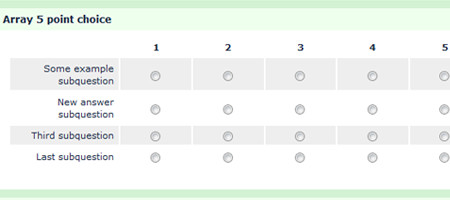
\psfig{file=screenshots/A.png}}}
\captionof{figure}{Matriz, elegir del 1 al 5}
\par


\subsection {Matriz (Elegir del 1 al 10)}
Este es un ejemplo, con la misma pregunta anterior, pero la escala de selecci'on es del 1 al 10.\\
\par
\centerline{\hbox{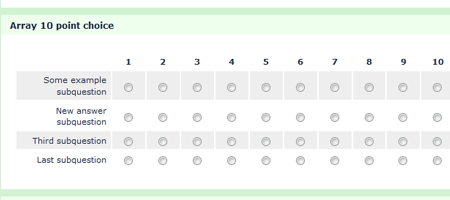
\psfig{file=screenshots/B.png}}}
\captionof{figure}{Matriz, elegir del 1 al 10}
\par 

\newpage
\subsection{Matriz de doble escala}

El tipo de pregunta Matriz de doble escala, permite dos escalas de opciones de pregunta para cada subpregunta, tal como se muestra en el siguiente ejemplo:\\
\par
\centerline{\hbox{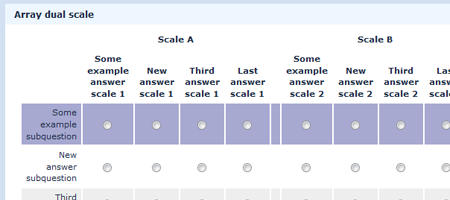
\psfig{file=screenshots/1.png}}}
\captionof{figure}{Matriz de doble escala}
\par

\subsection {G'enero}

\par
\centerline{\hbox{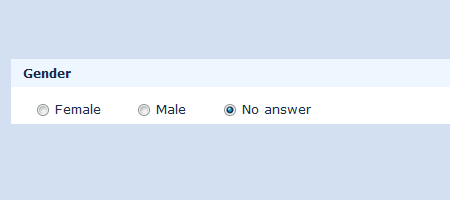
\psfig{file=screenshots/G.png}}}
\captionof{figure}{Matriz, elegir del 1 al 10}
\par

\subsection {Entrada num'erica}
Limita la entrada a un n'umero y un punto.
\par
\centerline{\hbox{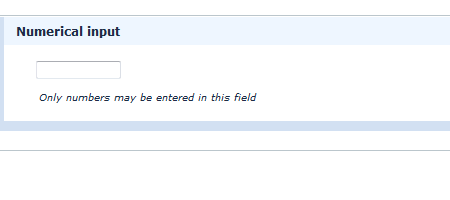
\psfig{file=screenshots/N.png}}}
\captionof{figure}{Entrada num'erica}
\par

\subsection {Listas de radio}
Listas de radio que pueden ser definidas en varias columnas.\\
\par
\centerline{\hbox{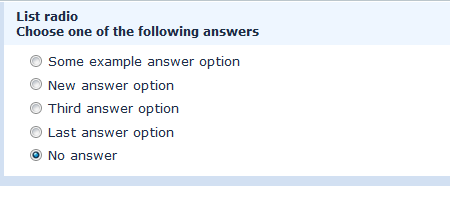
\psfig{file=screenshots/L.png}}}
\captionof{figure}{Listas de radio}
\par

\subsection {Entradas de texto libre}
Nos permite ingresar texto a nuestro gusto dependiendo del tama'no de la selecci'on.\\
\par
\centerline{\hbox{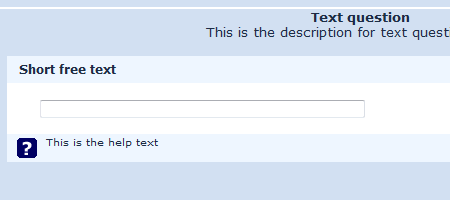
\psfig{file=screenshots/S1.png}}}
\captionof{figure}{Entrada de texto corto}
\par

\subsection {Entradas de texto libre largo}
\par
\centerline{\hbox{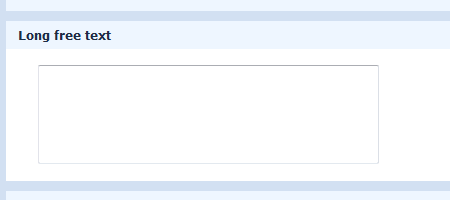
\psfig{file=screenshots/T.png}}}
\captionof{figure}{Entrada de texto largo}
\par

\subsection {Entradas de texto libre enorme}
\par
\centerline{\hbox{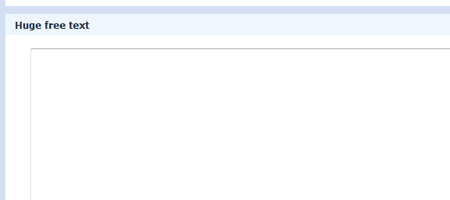
\psfig{file=screenshots/U.png}}}
\captionof{figure}{Entrada de texto enorme}
\par

Para mas informaci'on sobre tipos de entrada, se puede consultar la p'agina de Limesurvey.\footnote{http://docs.limesurvey.org/Tipos+de+preguntas\&structure=Manual+de+Instrucciones+en+Espa'nol}
\newpage

\subsection {Activando una encuesta}

Una vez que hayamos agregado nuestras preguntas, es momento de activar nuestra encuesta, para ello disponemos de un bot'on como lo demuestra la siguiente imagen:
\par
\centerline{\hbox{
\psfig{file=icons/inactive.png}
\psfig{file=icons/activate.png}}}
\captionof{figure}{Activaci'on de la encuesta}
\par 

Dando click sobre este bot'on vamos a iniciar el proceso de activaci'on de nuestra encuenta.

A continuaci'on nos har'a unas preguntas las cuales debemos contestar de la siguiente manera:
\par
\centerline{\hbox{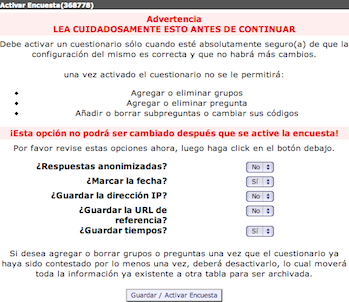
\psfig{file=screenshots/activating.png}}}
\captionof{figure}{Activaci'on de la encuesta}
\par 


Una vez activada la encuesta nos ense'ar'a la siguiente pantalla:
\par
\centerline{\hbox{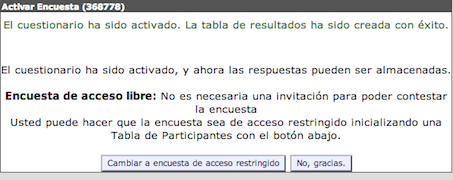
\psfig{file=screenshots/activating2.png}}}
\captionof{figure}{Activaci'on de la encuesta}
\par 

La cual nuestra respuesta ser'a que ``No, gracias'.', ya que de lo contrario necesitaremos ingresar los datos de las personas a encuestar, las cuales no disponemos de dicha informaci'on.

\section {Cuotas}
Para ingresar al apartado de cuotas, es necesario dar click en nuestro 'icono de "Propiedades de la encuesta'' y posteriormente en el 'icono de cuotas 
\psfig{file=icons/quota.png}

\subsection{Agregar una nueva cuota}
Para agregar una nueva cuota, debemos click al bot'on 
\psfig{file=screenshots/nueva_cuota.png}, por lo cual nos desplegara un formulario que nos pedir'a la siguiente informaci'on:
\par
\centerline{\hbox{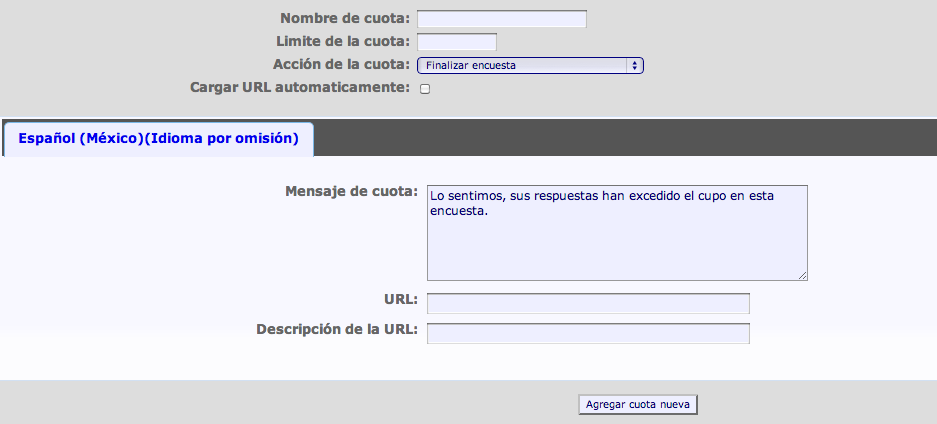
\psfig{file=screenshots/form_nueva_cuota.png,height=4.0in,width=7.0in}}}
\captionof{figure}{Activaci'on de la encuesta}
\par 


% FIN DEL DOCUMENTO
\end{document}


